\subsubsection{Blind Assignment for Blockchain Extension (BABE)}
\label{sec:babe}

In Polkadot, we produce relay chain blocks using our Blind Assignment for Blockchain Extension protocol (BABE).
 %\eray{, abbreviated BABE}{(BABE)}.
BABE assigns validators randomly to block production slots using  the randomness generated with blocks. A block production slot is a division of time when a block producer may produce a block. Note, that time is not universally agreed on, which we will address later.  These assignments are completely private until the assigned validators produce their blocks. Therefore, we use ``Blind Assignment'' in the protocol name. BABE is similar to Ouroboros Praos \cite{Praos} with some significant differences in the chain selection rule and timing assumptions.

In BABE, we may have slots without any assignment
%\eray{c}{assinments,}
 which we call empty slot. 
%\eray{slot}{slots}.
In order to fill the empty slots, we have a
%\eray{}{a}
secondary block production mechanism based on Aura \cite{aura} that assigns validators to slots publicly. We note that these blocks do not contribute to
%\eray{}{to} 
the security of BABE since the best chain selection and the random number generation algorithms work as if Aura blocks do not exist.
%\eray{the randomness generation \eray{do}{does} not consider randomness in the Aura blocks.}{-comment:I didn't understand this sentence.-}
Therefore, next we only describe BABE together with its security properties.
%since Aura blocks \eray{is}{are} not the part of the security of BABE.


BABE \cite{babe} consists of another time division called \emph{epochs} ($e_1,e_2,...$), where each epoch consists of a number of sequential block production slots (\(e_i = \{sl^i_{1}, sl^i_{2},\ldots,sl^i_{t}\}\)) up to the bound  $R$.
Each validator knows in which slots it is supposed to produce a block at the beginning of every epoch. When the time for its slot comes, the validator produces the block by proving that it is assigned to
%\eray{}{to} 
this slot.

The blind assignment is based on the cryptographic primitive called verifiable random function (VRF) \cite{vrf} (see Section \ref{sec:session_keys}). 
A validator in an epoch $e_m$  does the following to learn if it is eligible to produce a block in slot $sl_i^m$:
\begin{enumerate}
	\item  it obtains the randomness in the genesis block if $ m = 1  $ or $ m =2 $. Otherwise, it obtains the randomness  generated two epochs before ($e_{m-2}$).
	\item  it runs the VRF with its secret key and the input:  randomness and the slot number $ sl_i^m $.
\end{enumerate}

If the output of  VRF is less than the threshold $ \tau $, then the validator is the slot leader meaning that it is eligible to produce a block for this slot. We select $\tau$ with respect to security requirements of BABE \cite{babe} e.g., bigger $ \tau $ makes less probable to select only honest validators for a slot than smaller $ \tau $. 
When a validator produces a block, it adds the output of the VRF and its proof to the block which shows that its VRF output is less than $\tau$  in order to convince other validators that it has a right to produce a block in the corresponding slot. The validators always generate their blocks on top of the best chain.
The best chain selection rule in BABE says that ignore the Aura blocks and select the longest chain that includes the last finalised GRANDPA block. See Section \ref{sec:grandpa} for the details how blocks are finalised in GRANDPA.

The randomness of an epoch $e_m$ where $ m > 2 $ is generated by using the BABE blocks of the best chain that belongs to that epoch: let \(\rho\) be the concatenation of all  VRF values in BABE blocks that belongs to $e_m$. Then, compute the randomness for epoch $ e_m $ as $r_{m} = H(m
||\rho)$ where $ H $ is a hash function. Validators run periodically the relative time algorithm described below to learn at what time a slot starts according to their local clocks.




\paragraph{Relative Time Protocol:}

The elected validators for a slot need to know when the right time is to produce a block for the consistency and the security of BABE. For this, validators uses their local computer clock which is not adjusted by  any centralized clock adjustment protocols such as the Network Time Protocol \cite{ntp}. Instead, they keep their clock synchronised with the other validators with the relative time protocol. 
% \eray{when actually the right time to produce a block for the consistency and the security of the block production mechanism}{-comment:This sentence does not have a verb-}.
%For this purpose, they run the relative time protocol which lets them know when approximately a slot starts even if some clock drifts exist in their local clock. We note that in BABE, we do not rely on any centralized clock adjustment protocols such as the Network Time Protocol \cite{ntp}. 
%Therefore, we design the relative time protocol that depends on the arrival time of blocks according to local clocks of validators. 
%\eray{``Relative Time''}{``relative time protocol"}.
The formal security model of local clock synchronisation in blockchains without NTP and further details about the relative time protocol can be found in \cite{consensusonclock}.
%\eray{Please see \cite{consensusonclock} for the formal security model of synchronization in blockchains and for further details about the relative time protocol.}{The formal security model of synchronization in blockchains and further details about the relative time protocol can be found in \cite{consensusonclock}.}

In BABE, we assume that after the genesis block is released, elected validators of the first epoch store the arrival time of the genesis block with respect to their local clock. Then, they mark the beginning
 time of the first slot and increment
the slot number every $ T $ seconds. After this point,  they periodically run the relative algorithm not to lose the synchronisation with others because of their local clock drifts.  In addition to this, a validator who
joins after the genesis block runs the relative time algorithm to be synchronised with the other validators.

In every sync-epochs (different than epochs in BABE), validators update their clock according to the result of the relative time protocol and use the new clock until the next sync-epoch. The first sync-epoch $\varepsilon_1$ starts just after the genesis block is released. The other sync-epochs  $\varepsilon_i$ start when the slot number of the last (probabilistically) finalised block is $\bar{sl}_{\epsilon}$ which is the smallest slot number such that  $\bar{sl}_{\varepsilon} - \bar{sl}_{\varepsilon-1} \geq s_{cd}$ where $\bar{sl}_{\varepsilon-1}$ is the slot number of the last (probabilistically) finalized block in sync-epoch $\varepsilon-1$. Here, $s_{cd}$ is the parameter of the chain density (CD) property which will be defined according the chain growth.
In more detail, each validator  stores  the arrival time $ t_j $ of  blocks together with the slot number $\slot'_j$ in the block during a sync-epoch. At the end of a sync-epoch, the validator retrieves the arrival time of probabilistically finalized blocks generated during the sync-epoch and computes some candidate start times of the first slot $ \slot $ of the next sync-epoch i.e,  given that $ a_j = T(\slot - \slot'_j)  $,  $\mathcal{C}_T = \{t_j+a_j \}$. The times in $ \mathcal{C}_T $ are considered as candidates. In order to  choose one candidate,  the validator then sorts the list of candidates $ \mathcal{C}_T $ and outputs the median of the sorted list as a start time of the $ \slot $. An example execution of the relative time protocol in the first sync-epoch is in Figure \ref{fig:relativetime}.

\begin{figure}[h]
	\centering
	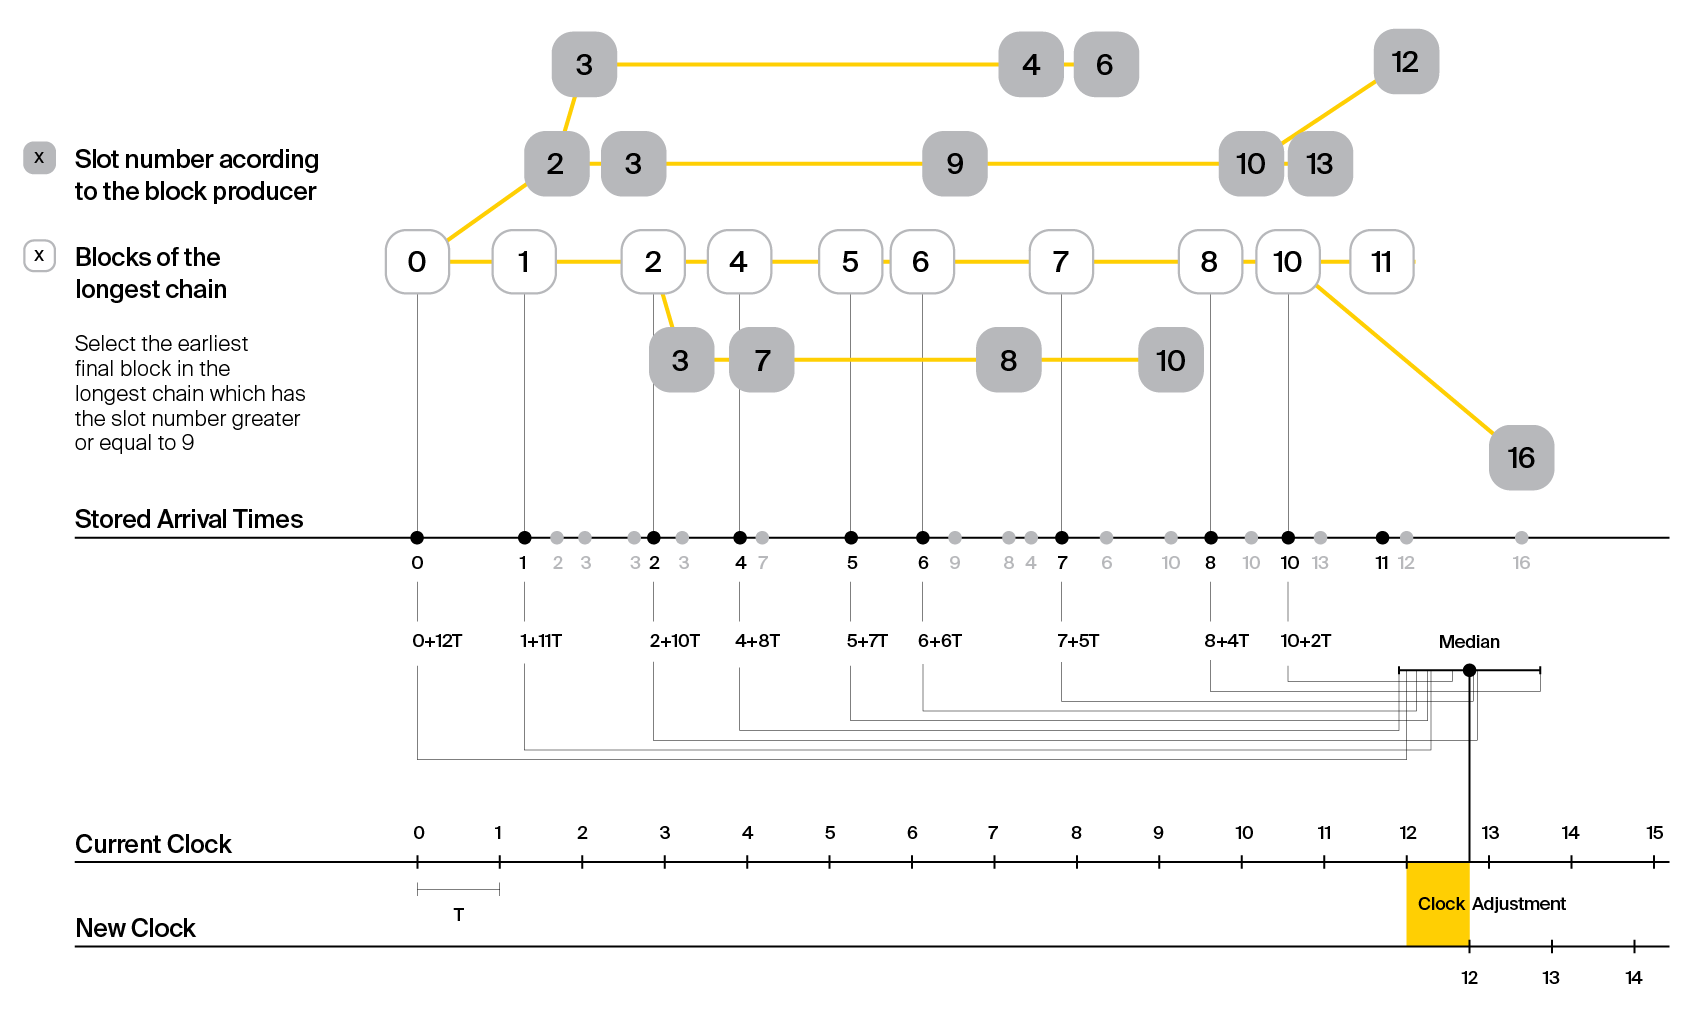
\includegraphics[width=1.\textwidth]{images/BABE3.png}
	\caption{An example execution of the relative time protocol in the first epoch where $s_{cd} = 9$}
	\label{fig:relativetime}
\end{figure}



\paragraph{Security Overview of BABE:} Garay et al. \cite{backbone} define the properties below in order to obtain a secure blockchain protocol. Informally, we can describe these properties as follows:

\begin{itemize}
	\item \emph{Common Prefix (CP):} \label{item:common_prefix}
	%\eray{}{-comment: Isn't this CPP? How did you get CP as an abbreviation here?-}:}: It is used as CP in the literature. I removed the Property to be consisten with the name of the next properties
	 It ensures that the blocks which are $ k $-blocks before the last block of an honest validator's blockchain cannot be changed. We call  all unchangeable blocks  \emph{finalized} blocks. BABE satisfies CP property thanks to the honest super majority since malicious validators are selected for a slot probabilistically much less than the honest validators. It means that malicious validators do
	 % \eray{does}{do}
	  not have enough 
	  %\eray{source}{sources}: source sounds better for me
	  to construct another chain which does not include one of the finalised blocks.
	\item \emph{Chain Quality (CQ):} \label{item:chain_quality} It ensures a minimum honest block contribution to any best chain owned by an honest party in every certain number of slots. We guarantee even in the worst case where a network delay is maximum that there will be at least one honest block in the best chain during an epoch so that the randomness cannot be biased.
	\item \emph{Chain Growth (CG):} \label{item:chain_growth} It guarantees a minimum growth between slots. Thanks to super majority of honest validators, malicious validators cannot prevent the growth of the best chain.
	
	\item \emph{Chain Density (CD):} \label{item:chain_density} It ensures that in a sufficiently long portion of the best chain more than half of the blocks produced by honest validators. CQ and CG properties %\eray{implies}{imply} 
	imply this property \cite{Praos}.
\end{itemize}
Further details about BABE and  its security analysis can be found in \cite{babe}.

%\eray{Please see \cite{babe} for further details about BABE and  its security analysis.}{Further details about BABE and  its security analysis can be found in \cite{babe}.}
